\chapter{CONCLUSIONS}


\section{Higher power in Enhanced LIGO}
The broad result of the Input Optics and Angular Sensing and Control
upgrades along with the work of many other people on many other
subsystems was successful operation of both the Hanford and Livingston
interferometers at the highest of laser powers ever used. The typical
input powers used during Initial LIGO were between 5 and 7~W and
during Enhanced LIGO typical input powers were between 8 and 20~W, as
shown by the histograms in Figure~\ref{fig:S6pwrs}. 

\begin{figure}
\begin{centering}
\subfigure{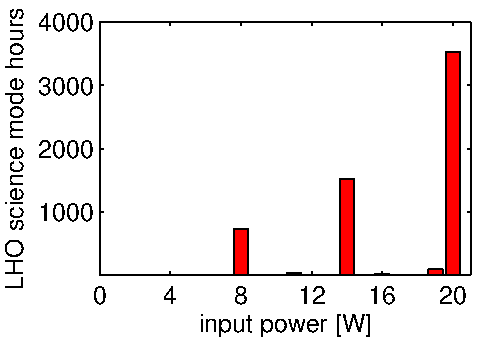
\includegraphics{figures/thesisS6pwrs_LHO.pdf}}\subfigure{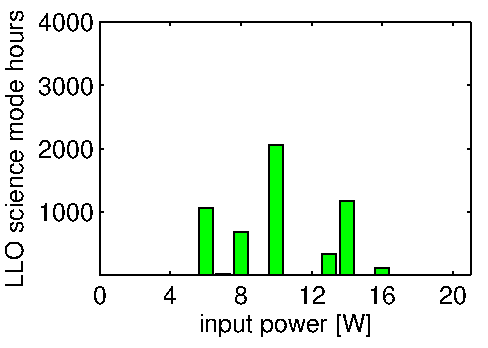
\includegraphics{figures/thesisS6pwrs_LLO.pdf}}
\caption[Histogram of input powers used during S6]{Histogram of input
  powers used during S6 at each site.}
\label{fig:S6pwrs}
\end{centering}
\end{figure}

A snapshot of how the interferometer reacts to increases in laser
power is found in Figure \ref{fig:striptool}, which shows the time
series of several channels during a typical lock loss and re-lock of
the interferometer followed by an increase in input power to 14~W. The
increase in the fluctuations of NSPOB, the sideband power in the PRC,
prior to the lock loss at $t=250$ sec indicates PRC instability. The
MC regains lock almost immediately and the power is increased to
1~W. The dense region of NSPOB signal shows the flashes of resonance
as the interferometer tries to acquire lock, which it ultimately does
at around $t=500$~sec. The laser power is subsequently increased to
8~W, and pulses of TCS power turned on to hasten the ITM cooling
process in preparation for the laser power increase to 14~W. All
along, the power in the arm cavities increases as well as that
reflected from the interferometer. NSPOB is a bit more ``hairy'' at
14~W than it is at 8~W, but this lock is otherwise stable and provides
a neutron star binary inspiral range of 15~Mpc and lasts for 5 hours
until an earthquake kills it.

\begin{figure}
\begin{centering}
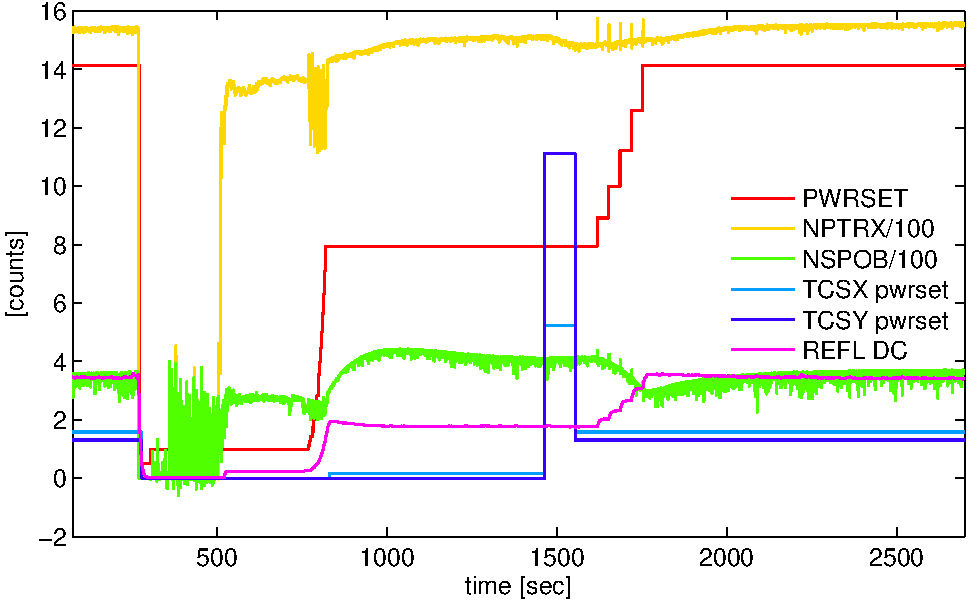
\includegraphics[width=1.0\columnwidth]{figures/timeseries_ifolocked.pdf}
\caption[Time series of interferometer signals showing a typical lock
loss and re-lock followed by an increase of power to 14~W]{Time series
  of interferometer signals showing a typical lock loss (at about 250
  sec) and re-lock (at about 500 sec) followed by an increase of power
  to 14~W. The y-axis is in units of Watts for the input power, TCSX,
  and TCSY traces. The other traces are displayed in digital
  counts. Data is from July 23, 2009.}
\label{fig:striptool}
\end{centering}
\end{figure}

The improvement in strain sensitivity in the shot-noise-limited region
due to operating at higher laser power is seen in
Figure~\ref{fig:LIGOcurves}. There is a factor of two improvement from
Initial LIGO to Enhanced LIGO from about 300~Hz on. The corresponding
best neutron star binary range increased from 15 to 20~Mpc. Although
more power improves the shot-noise-limited region of the strain
spectrum, it does introduce many complications for interferometer
operation that must be carefully addressed.

\begin{figure}
\begin{centering}
\includegraphics{figures/LIGOcurves_zoom.pdf}
\caption[Zoom of the shot-noise-limited noise floors of the Initial
LIGO and Enhanced LIGO detectors.]{Zoom of the shot-noise-limited
  noise floors of the Initial LIGO and Enhanced LIGO detectors. The
  improved Input Optics and Angular Sensing and Control enabled the
  increase in power for Enhanced LIGO. The shot-noise-limited strain
  sensitivity improved by a factor of two.}
\label{fig:LIGOcurves}
\end{centering}
\end{figure}


\section{Summary}
We described the design of the Enhanced LIGO Input Optics and Angular
Sensing and Control subsystems and presented measurements
characterizing the systems and their performances when operating with
record laser powers. Upgrades to the two systems were necessary for
allowing higher laser powers, for improving the efficiency of sending
light into the interferometer, and for keeping light in the
interferometer once it is there. Higher power in the interferometer
improves the shot-noise-limited noise floor, and we succeeded at
operating the interferometers with more than twice the highest of
powers achievable during Initial LIGO. The Enhanced LIGO
shot-noise-limited sensitivity did indeed reach record levels,
improving the chances of gravitational-wave detection.

In addition, we directly measured the stable and unstable
opto-mechanical modes of the Fabry-Perot arm cavities. We witness the
expected effect of radiation pressure torque, demonstrating a clear
understanding of the physics that will affect future generations of
laser interferometers for gravitational-wave detection. Furthermore,
we successfully controlled the stable and unstable opto-mechanical
modes without contaminating the gravitational-wave readout in the
frequency range of interest.



%\the\columnwidth